\section{CTFEF}

\begin{frame}
    \frametitle{CTFEF compiler architecture}
    \begin{figure}
        
        \begin{center}
            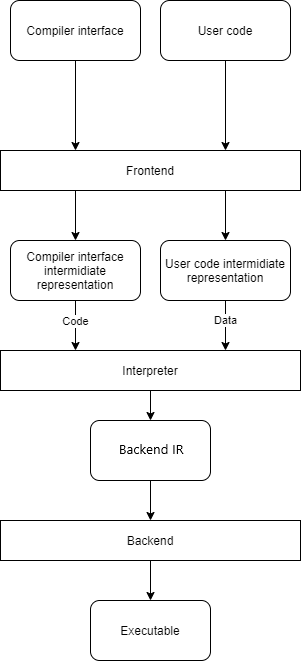
\includegraphics[height=6cm]{pictures/compiler-structure.png}
        \end{center}
    \end{figure}

\end{frame}


\begin{frame}
    \frametitle{Frontend}

    \begin{itemize}
        \item Translates source code into Intermediate Representation\begin{itemize}
            \item Parse
            \item Validate syntax
            \item Inline operators with special syntax (ex: \lstinline|typeof|)
        \end{itemize}
        \item Processes user code and Compiler Interface \begin{itemize}
            \item Compiler Interface translates user code into backend Intermediate Representation
        \end{itemize}
        \item May perform additional processing\begin{itemize}
            \item In C-=-1 it invokes the interpreter to execute metaprogramming code
        \end{itemize}
    \end{itemize}

\end{frame}

\begin{frame}
    \frametitle{Intermediate Representation}

    \begin{itemize}
        \item Complete representation of the user program
        \item Simplified form of the compiled language\begin{itemize}
            \item Resolved function overloads
            \item Advanced constructs lowered to basic ones (foreach loops transformed into while)
        \end{itemize}
        \item Stored using Interpreter data structures in compiler memory\begin{itemize}
            \item Reduces the need for marshalling between interpreted code and the compiler
            \item Introduces significant amount of indirection to all data structures
        \end{itemize}
    \end{itemize}

\end{frame}

\begin{frame}
    \frametitle{Interpreter}

    \begin{itemize}
        \item Operates on Intermediate Representation 
        \item Uses the same data structures for code and data
        \item Allows executing arbitrary code \begin{itemize}
            \item In practice some operations make sens only at runtime
            \item Some operations must be done slightly differently between runtime and compiletime (ex: memory management)
        \end{itemize}
        \item Must expose api for generating backend IR\begin{itemize}
            \item In case of C-=-1 bindings for parts of LLVM library were created
        \end{itemize}
    \end{itemize}

\end{frame}

\begin{frame}
    \frametitle{Backend}

    \begin{itemize}
        \item Module that generates machine code based on IR generated by Compiler Interface
        \item No constraints are placed on this module by CTFEF architecture
        \item In case of C-=-1 compiler, LLVM library was used without any modifications
    \end{itemize}

\end{frame}
